\input{src/header}											% bindet Header ein (WICHTIG)
\usepackage{graphicx}
\usepackage{fancyvrb}

\newcommand{\dozent}{Prof. Dr. Agn`es Voisard, Nicolas Lehmann}					% <-- Names des Dozenten eintragen
\newcommand{\tutor}{Nicolas Lehmann}						% <-- Name eurer Tutoriun eintragen
\newcommand{\tutoriumNo}{6}				% <-- Nummer im KVV nachschauen
\newcommand{\projectNo}{2}									% <-- Nummer des Übungszettels
\newcommand{\veranstaltung}{Datenbanksysteme}	% <-- Name der Lehrveranstaltung eintragen
\newcommand{\semester}{SoSe 2017}						% <-- z.B. SoSe 17, WiSe 17/18
\newcommand{\studenten}{Boyan Hristov, Julian Habib}			% <-- Hier eure Namen eintragen
% /////////////////////// BEGIN DOKUMENT /////////////////////////


\begin{document}
% /////////////////////// BEGIN TITLEPAGE /////////////////////////
\begin{titlepage}
	\subject{\dozent}
	\title{\veranstaltung, \semester}
	\subtitle{\Large Übungsblatt \projectNo\\ \large\vspace{1ex} }
	\author{\studenten}
	\date{\normalsize \today}
\end{titlepage}

\maketitle								% Erstellt das Titelblatt
\vspace*{-9cm}							% rückt Logo an den oberen Seitenrand
\makebox[\dimexpr\textwidth+1cm][r]{	%rechtsbündig und geht rechts 1cm über Layout hinaus
	\includegraphics[width=0.4\textwidth]{src/fu_logo} % fügt FU-Logo ein
}
% /////////////////////// END TITLEPAGE /////////////////////////

\vspace{7cm}							% Abstand
\rule{\linewidth}{0.8pt}				% horizontale Linie										% erstellt die Titelseite


Link zum Git Repository: \url{https://github.com/BoyanH}

% /////////////////////// Aufgabe 1 /////////////////////////
\section{Aufgabe}


\begin{itemize}

\item[a)]

Relationales Modell \\

% Relational Modell
\begin{Verbatim}[commandchars=+\[\]]

Person(+underline[ID::integer], Age::integer, Name::character varying(20), Password::character varying(40),
	Login::character varying(40))
Teacher(+underline[ID::integer])
Student(+underline[ID::integer])
Course(+underline[Number::integer], Name :: character varying(50))
Module(+underline[Number::integer], Name :: character varying(50))

PersonIsATeacher(+underline[PersonID, TeacherID])
PersonIsAStudent(+underline[PersonID, StudentID])
TeachesCourses(+underline[PersonID, CourseNumber], InSemester)
ContainsCourses(+underline[ModuleNumber, CourseNumber])
AttendsCourses(+underline[StudentID, CourseNumber])
\end{Verbatim}
% End of relational Modell

ER Diagramm in umgekehrter min-max Chen Notation \\

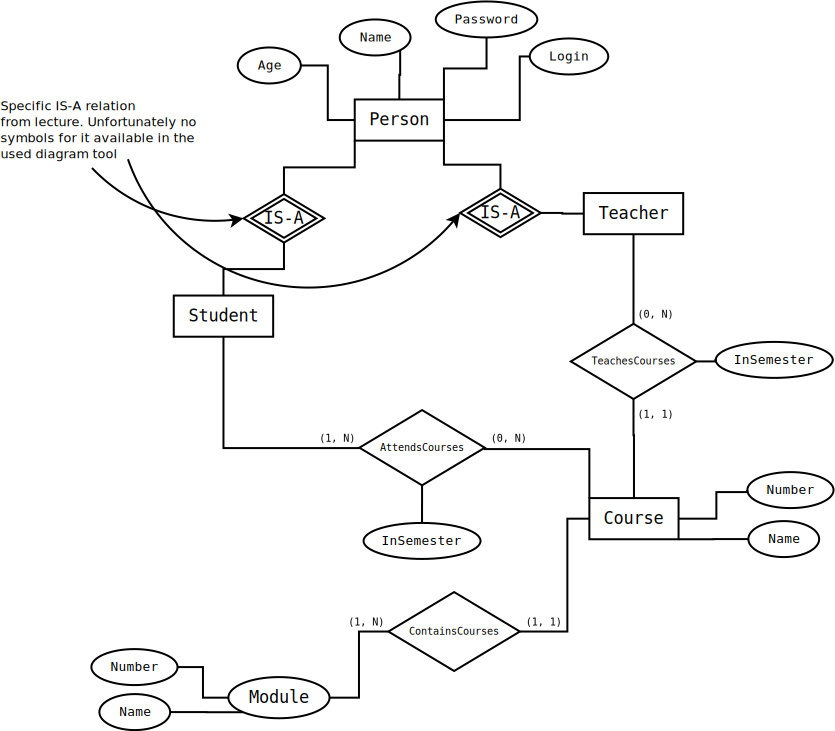
\includegraphics[width=\textwidth]{./src/exercise3_A.png}


\item[b)] 

Relationales Modell \\

% Relational Modell
\begin{Verbatim}[commandchars=+\[\]]

Person(+underline[ID::integer], Name::character varying(20))
Doctor(+underline[ID::integer], Specialty::character varying(30), Name::character varying(20))
Patient(+underline[ID::integer], HealthHistory::character varying(40) ARRAY, Name::character varying(20))
DoctorsAppointment(+underline[ID::integer], Date::date)
Address(+underline[PrivateAddressStreet::character varying(20)], City::character varying(20), 
	ServiceAddressStreet::character varying(20))

LivesIn(+underline[PersonID, AddressPrivateAdressStreet])
Attends(+underline[PersonID, DoctorsAppointmentID])
Services(+underline[PersonID, DoctorsAppointmentID])
\end{Verbatim}
% End of relational Modell

ER Diagramm in umgekehrter min-max Chen Notation\\

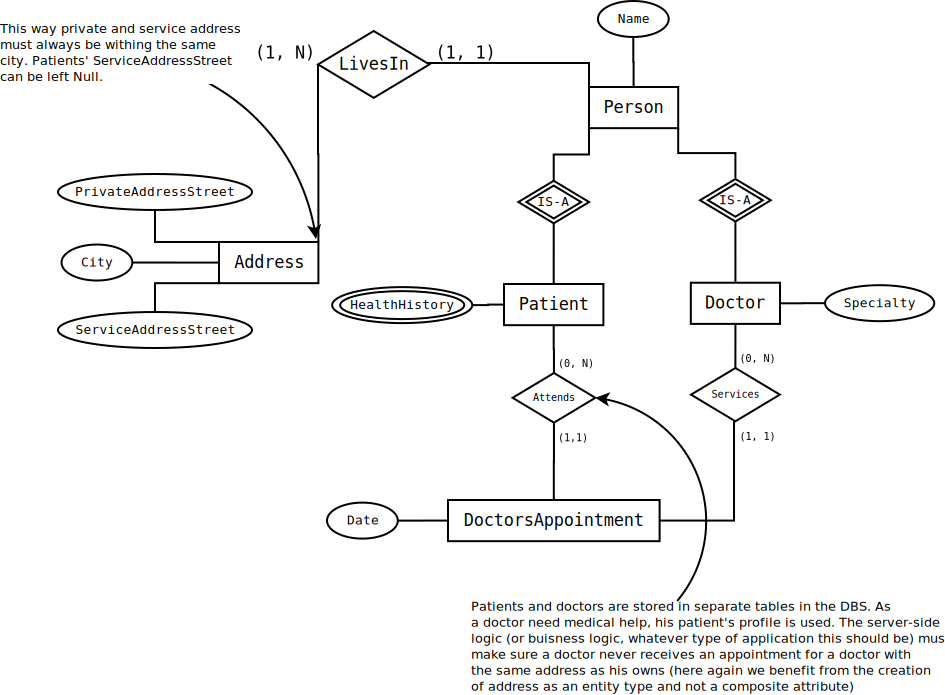
\includegraphics[width=\textwidth]{./src/exercise3_B.png}

\end{itemize}

\section{Aufgabe}

\begin{itemize}


\item[a)]
$\Pi_{\text{Vorname, Nachname}}$ ($\sigma_{\text{Alter} < 30 }$)

\item[b)]
$\Pi_{\text{Datum}}$ ($\sigma_{\text{Temperatur > Regenmenge } \lor \text{ Temperatur > Sonnenscheindauer} }$)

\item[c)]
$\Pi_{\text{Kreditkartennummer}}$ ($\sigma_{\text{Name = 'Emirates' $\land$ Datum $\geq$ '02.03.2016' $\land$ Datum $\leq$ '07.06.2016'}}$  (Passagier $\bowtie_{\text{ID = Passagier-ID}}$ Flug $\bowtie_{\text{Fluggesellschaft-ID = ID}}$ Fluggesellschaft))

\item[d)]
$\Pi_{\text{Name}}$ ($\sigma_{\text{Temperatur < 0}}$ (Wetter $\bowtie_{\text{Wetter::Datum = Flug::Datum}}$ Flug $\bowtie_{\text{Fluggesellschaft-ID = ID}}$ Fluggesellschaft))

\item[e)]
$\Pi_{\text{Vorname, Nachname}}$ ($\sigma_{\neg\text{(Temperatur < 20 $\land$ Regenmenge > 10 $\land$ Sonnenscheindauer < 6)}}$ (Wetter $\bowtie_{\text{Wetter::Datum = Flug::Datum}}$ Flug $\bowtie_{\text{Passagier-ID = ID}}$ Passagier))

\end{itemize}




% /////////////////////// END DOKUMENT /////////////////////////
\end{document}